\documentclass[11pt,draft,phd]{osudiss-2} 

\usepackage[english]{babel}
\usepackage{microtype}
\usepackage{amsmath}
\usepackage[numbers,sort&compress]{natbib}
\usepackage{doi}
\usepackage{graphicx}
\usepackage{tabularx}
\usepackage{dcolumn}
\usepackage{booktabs}
\usepackage{scrextend} % for \footref
\usepackage{hyperref}
\usepackage[nameinlink,capitalize]{cleveref}
\usepackage{siunitx}
\usepackage{enumitem}
\usepackage{floatrow}
\usepackage{bm}

%\usepackage[acronym, section=chapter]{glossaries}
%\makeglossaries
%\include{acronyms}

\usepackage{lipsum}

% style stuff
\bibliographystyle{apsrev4-1-custom}
\addto{\captionsenglish}{\renewcommand{\bibname}{References}}
\hypersetup{hidelinks}

% custom commands
\DeclareMathOperator{\Tanh}{\mathbf{tanh}}

% use dcolumn
\newcolumntype{d}{D{.}{.}{-1}}

\title{Essential Reservoir Computing}
\author{Aaron Griffith}
\advisorname{Daniel J. Gauthier}
\degree{Doctor of Philosophy}
\member{Amy Connolly}
\member{Ciriyam Jayaprakash}
\member{Gregory Lafyatis}
\authordegrees{B.S.}
\graduationyear{2021}
\unit{Graduate Program in Physics}

\begin{document}

\frontmatter

\begin{abstract}
  % FIXME abstract
  An abstract goes here. It should be less than \textbf{500 words}.
\end{abstract}

\dedication{For my parents Gregory and Mary Lea, and my brother Nathan.}

\begin{acknowledgments}
  This work would not have been possible without the committed support
  of my advisor, Daniel J. Gauthier, or my insightful collaborators,
  including Wendson A.~S. Barbosa, Erik Bollt, Daniel Canaday, and Andrew
  Pomerance.

  In addition, many discussions over the years have
  re-contextualized my understanding of reservoir computers. I would
  specifically like to thank Michelle Girvan, Edward Ott, and Brian Hunt.
\end{acknowledgments}

\begin{vita}
  \dateitem{2009-2014}{B.S., Mathematics and Physics \\ The Ohio State University}
  \dateitem{2015-2016}{Graduate Teaching Associate \\ Department of Physics \\ The Ohio State University}
  \dateitem{2016-2021}{Graduate Research Associate \\ Department of Physics \\ The Ohio State University}

  \begin{publist}
    \pubitem{D.~Canaday, A.~Griffith, and D.~J.~Gauthier, ``Rapid time series prediction with a hardware-based reservoir computer,'' \href{https://doi.org/10.1063/1.5048199}{Chaos: An Interdisciplinary Journal of Nonlinear Science \textbf{28}, 123119 (2018)}.}
    \pubitem{A.~Griffith, A.~Pomerance, and D.~J.~Gauthier, ``Forecasting chaotic systems with very low connectivity reservoir computers,'' \href{https://doi.org/10.1063/1.5120710}{Chaos: An Interdisciplinary Journal of Nonlinear Science \textbf{29}, 123108 (2019)}.}
    \pubitem{W.~A.~S.~Barbosa, A.~Griffith, G.~E.~Rowlands, L.~C.~G.~Govia, G.~J.~Ribeill, M.-H.~Nguyen, T.~A.~Ohki, and D.~J.~Gauthier, ``Symmetry-aware reservoir computing,'' \href{https://arxiv.org/abs/2102.00310}{(2021), \\ arXiv:2102.00310 [cs.NE]}.}
    \pubitem{D.~J.~Gauthier, E.~Bollt, A.~Griffith, W.~A.~S.~Barbosa, ``Next generation reservoir computing,'' \href{https://arxiv.org/abs/2106.07688}{(2021), arXiv:2106.07688 [cs.LG]}.}
  \end{publist}

  \begin{fieldsstudy}
    \majorfield{Physics}
  \end{fieldsstudy}
\end{vita}

\tableofcontents 

\clearpage
\listoffigures 

\clearpage
\listoftables 

%\clearpage
%\PrintListofAbbreviations{List of Abbreviations}

\mainmatter
\chapter{Introduction}\label{ch:introduction}

% Goals:
% - contextualize RC in physics
% - new field, interest, ML physics
% - outline rest, put important figures in intro
% - who helped and what did I do

Recently, many difficult problems have been solved using methods from
the field of machine learning, in particular using neural
networks. Machine learning methods work by learning solutions from
example data alone, without the need for an existing model for that
data.  Physicists have used neural networks to find the masses of
particles from decay data~\cite{lonnblad1992} and separate quark and
gluon jets in $e^+ e^-$ annihilation~\cite{csabai1991}.  In other
fields, this approach has been used effectively on handwritten digit
recognition~\cite{lecun1998,simard2003}, speech
recognition~\cite{hinton2012}, and speech production~\cite{oord2016}.
These are all problems with large sets of example data, but which are
otherwise difficult or intractable with a more traditional programming
approach. Put simply, it is easy to provide examples of what the
number ``\num{2}'' looks like, while it is difficult to define what
features a written ``\num{2}'' must have in a programming language.

By its nature, many problems in physics are defined in terms of
time-varying data. Neural networks that contain internal cycles,
called recurrent neural networks, are a natural fit for these
problems. The addition of cycles gives the resulting network memory
and allows it to be used to effectively solve many time-domain
problems, such as forecasting chaotic
systems~\cite{garcia-pedrero2010}. However, this modification has a
cost: recurrent neural networks take much more time to train, as the
training algorithm takes exponentially longer to learn how to utilize
past inputs~\cite{bengio1994,lukosevicius2009}.

More recently, a new machine learning tool has emerged for dealing
with time-domain problems.  Known as \emph{reservoir computing}, this
tool was originally formulated as a novel way to reduce the
computational cost of training recurrent neural
networks~\cite{lukosevicius2009}. Reservoir computers (RCs) have been
effectively applied to chaotic system
forecasting~\cite{jaeger1978,pathak2017}, system state
inference~\cite{lu2017}. More than just short-term prediction, RCs are
capable of reproducing the \emph{climate} of a dynamical
system;~\cite{pathak2017,haluszczynski2019} it learns the long-term
features of the system, such as the system's attractor and Lyapunov
exponents.

RCs are interesting to physicists not only as a tool to solve
problems. At the heart of a RC is a dynamic system called the
\emph{reservoir}, which provides the rich dynamics the RC draws on to
function. This is usually implemented as a neural network, but in
practice many dynamic systems function well. This opens the door to
building RCs around real physical systems, such as a network of
autonomous logic on an FPGA~\cite{canaday2018} or an optical feedback
system~\cite{antonik2016}. This is interesting from a theoretical
perspective, as physical RCs use an ancillary system to help answer
questions about a main system, but they are also practically
interesting: by relying on physical reservoirs, rather than simulated,
these methods perform chaotic system forecasting at a very high rate.

As a new field, reservoir computing still has many unanswered
fundamental questions. What qualities should the internal reservoir
have to create a good RC? A common practice is to use a random network
as the reservoir, generated from a set of metaparameters. There are a
handful of results for some parameters, such as setting the
\emph{spectral radius} of the network near unity and the need for
recurrent network connections,\cite{jaeger2001,lukosevicius2012} but
the applicability of these results is narrow. What features of the
reservoir are necessary, and which can be discarded?

In this thesis, I will construct reservoir computers that do not
follow the conventional rules for reservoir construction. These RCs
continue to perform well on chaotic system forecasting and state
inference, and can even reproduce the chaotic attractor of the system
they have learned, despite the fact that their internal reservoir has
no recurrent connections. Indeed, by the end of this thesis, they do
not have an internal reservoir at all.

\section{Outline and Summary of Contributions}

%\begin{reusefigure}{fig:reservoir}
%  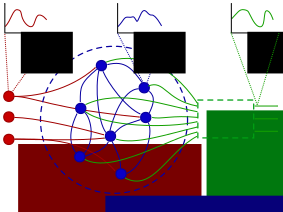
\includegraphics[width=0.6\textwidth]{figures/reservoir}
%  \caption{Re-used caption.}
%\end{reusefigure}

In \cref{ch:reservoir-computing}, I describe the reservoir computing
method, as well as a common concrete implementation of a RC called an
echo state network (ESN). I explain how to construct an ESN, the
metaparameters that govern its construction, and discuss some of the
limited known results for choosing these metaparameters. Then, I
discuss how the RC is trained, both for autonomous forecasting tasks
and for inference tasks, as well as how performance quality on these
tasks is commonly measured. I briefly discuss the known problems with
this performance measure, and suggest a few alternative methods.

In \cref{ch:low-connectivity}, I apply RCs to the task of chaotic
system forecasting for three different chaotic systems. I use a
Bayesian optimization algorithm to tune the metaparameters for the
RCs, and in so doing, discover a class of well-performing RCs with very
simple internal reservoirs. I identify four classes of reservoir
networks with simple structure. Two of these classes had been
previously identified. I build on this work and demonstrate that all
four classes have the capacity to perform as well as a traditional
RC. In particular, all four classes can reproduce the chaotic
attractor of the system they are trained on. I then discuss the
trade-offs between these simpler reservoir structures and a
traditional RC.

In \cref{ch:nvar} I describe a different technique known as
non-linear vector autoregression (NVAR), which has recently been shown
to be mathematically equivalent to an RC under certain conditions. I
discuss the construction and training of an NVAR, and how to apply it
to common RC tasks. Then, I discuss the parallells between the NVAR
and RC approaches, as well as when the equivalence is known to
hold. Finally, I discuss the tradeoffs between the two approaches.

In \cref{ch:nvar-application}, I build on this equivalence with my
collaborators to demonstrate NVARs solving two common RC tasks: system
forecasting and state inference. I show that NVARs are capable of
RC-equivalent performance on these tasks despite being considerably
simpler than an RC, and can achieve this performance with very little
training data and training time. In addition, I discuss how a trained
NVAR can provide interpretable results, while a trained RC is
opaque. I discuss how to move beyond the strict proven mathematical
equivalence to solve a wider variety of problems, and then demonstrate
this by performing chaotic system forecasting on a system without a
known equivalence.

%In \cref{ch:nvar-hardware}, I utilize the simplicity of the NVAR
%approach to implement it in hardware on an FPGA.
% FIXME you haven't done this yet

Finally, in \cref{ch:conclusion}, I summarize my findings and
contributions, and propose interesting new directions for future
research discovered during this work.

\chapter{Reservoir Computing}\label{ch:reservoir-computing}

At a high level, a \emph{reservoir computer} (RC) is a method to
transform one time-varying signal $\bm{u}(t)$, the input to the RC,
into another time-varying signal $\bm{y}(t)$, the output of the
RC. The RC is constructed in such a way that, given an example input
and a desired output, the RC can be \emph{trained} to produce that
output when given the corresponding input. Once trained, the RC can
then be used to perform the trained transformation on inputs it has
not seen before.

The RC does this by means of an internal dynamic system called the
\emph{reservoir}, which is coupled to the input $\bm{u}(t)$. If the
reservoir's dynamics can be expressed as a first-order differential
equation, which covers a broad range of interesting choices of
reservoir, then the reservoir's internal state $\bm{r}$ is given by
\begin{equation}
  \label{eq:reservoir}
  \dot{\mathbf{r}}(t) = \mathbf{R}\left(\mathbf{r}, \mathbf{u}, t\right),
\end{equation}
where $\mathbf{R}$ defines the dynamics of the reservoir.

The reservoir is commonly a specific type of system called an
\emph{echo state network}, discussed in \cref{sec:esn}, but this is
not at all a requirement. Effective RCs have been built around
autonomous Boolean networks~\cite{canaday2018}, optical feedback
systems~\cite{antonik2016}, single time-delay Boolean
nodes~\cite{haynes2015}, and many others. The specific properties that
a reservoir must have in order to produce a functioning RC is an open
question. Though there are a few known results, which I will discuss
in \cref{sec:reservoir-properties}, the most direct and practical way
to know if a given reservoir will work is to build, train, and test
it.

The output $\bm{y}(t)$ of the RC is a linear
combination of a set of \emph{read-out} signals, constructed from the
reservoir state $\bm{r}(t)$ by means of a read-out function $\bm{g}$:
\begin{equation}
  \label{eq:output}
  \bm{y}(t) = W_\text{out}\;\bm{g}\left(\bm{r}(t)\right).
\end{equation}
This is called the RCs \emph{output layer}. Often, $\bm{g}$ is the
identity function, and the output signal $\bm{y}(t)$ is a direct
linear combination of the state variables of the reservoir. However, a
non-identity $\bm{g}$ can be used to break unwanted symmetries in the
$\bm{u}$-to-$\bm{y}$ transformation, to introduce non-linearity to an
otherwise completely linear RC, or to model incomplete measurements of
a physical system being used as a reservoir.

% FIXME figure for generic reservoir

Together, \cref{eq:reservoir} and \cref{eq:output} define a reservoir
computer, and define the transformation from input signal $\bm{u}(t)$
to output $\bm{y}(t)$.

Intuitively, the input signal $\bm{u}(t)$ drives the reservoir,
producing a large number of reservoir state signals $\bm{r}(t)$. These
state signals may be quite complicated, and likely none of them match
the desired transformation, but they are combined by means of
$W_\text{out}$ to produce the desired transformation. The reservoir's
purpose is to broadcast the input signal into a high-dimensional
space, and the output layer's purpose is to combine those many dimensions
into the meaningful desired output of the RC.

The reservoir dynamics $\bm{R}$ and the readout function $\bm{g}$ are
considered a fixed part of the RCs construction, and are not part of
the training process. I will discuss this choice in more detail in
\cref{sec:esn,sec:reservoir-properties}. Once these design parameters
are fixed, the weight matrix $W_\text{out}$ can be calculated from an
example input and an example output by a process called
\emph{training}, which results in a complete RC that performs the desired
transformation.

\section{Training an RC}\label{sec:training}

Training an RC starts with an example input signal
$\bm{u}_\text{train}(t)$ and corresponding example output signal
$\bm{y}_\text{train}(t)$. As an example, $\bm{u}_\text{train}(t)$ might be
the $x$ and $y$ components of a three-dimensional dynamic system, and
$\bm{y}_\text{train}(t)$ would be the $z$ component. An RC trained on this
example would learn how to infer the $z$ component of the system from
the other two.

The first step is to feed the example input $\bm{u}_\text{train}(t)$ into the reservoir, producing an example reservoir response $\bm{r}_\text{train}(t)$. Using \cref{eq:output}, the final goal of training is to find a $W_\text{out}$ such that
\begin{equation}
  \label{eq:approx-output}
  \mathbf{y}_\text{train}(t) \approx W_\text{out}\;\mathbf{g}\left(\mathbf{r}_\text{train}(t)\right).
\end{equation}

For many practical reservoirs, it takes some time for the reservoir
state $\bm{r}(t)$ to synchronize with the input $\bm{u}(t)$. During
this time, the reservoir state still depends on its initial condition,
and so is unsuitable for use as training data. Practically, if the
example data starts at $t = 0$, then all the data before $t <
t_\text{warmup}$ is discarded, and the approximation in
\cref{eq:approx-output} need only be true for $t >
t_\text{warmup}$. The warm-up time $t_\text{warmup}$ will depend on the
specific choice of reservoir in the RC.

The right-hand side of \cref{eq:approx-output} is linear in
$W_\text{out}$, and can be solved by any number of linear regression
methods. For RCs, $W_\text{out}$ is most commonly found via ridge
regression, also known as Tikhonov regularization, which chooses
$W_\text{out}$ to minimize
\begin{equation}
  \label{eq:ridge}
  \alpha ||W_\text{out}||^2 + \sum_{t>t_\text{warmup}} |\mathbf{u}_\text{train}(t) - W_\text{out}\;\mathbf{r}_\text{train}(t)|^2.
\end{equation}
In most practical applications, the signals involved are either
measured at a fixed time step, or integrated at a fixed time step, and
the sum in \cref{eq:ridge} is understood to be over these fixed time
steps.

The ridge parameter $\alpha$ is included to prevent over-fitting, and
to help the RC generalize from the example input to unknown inputs. In
practice, this value depends on the scale of the input signal
$\bm{u}_\text{train}(t)$; for roughly unit-scale inputs, $\alpha$ may be
anywhere from $10^-{9}$ to $10^9$. Since the ridge regression can be
calculated quickly, and the result is only logarithmically sensitive
to the value of $\alpha$, the best value for $\alpha$ can be found
simply by grid search or cross-validation on the example input.

% FIXME better cite
The fact that training an RC amounts to a linear regression is a major
feature worth highlighting. Linear regressions are very fast, compared
to other machine learning techniques like gradient descent and
backpropogation~\cite{lukosevicius2009}. As a result, training an RC
is also fast. This opens the door to many interesting applications
where the ability to rapidly retrain the RC to a new system without the aid of
a supercomputer is desirable. For example, an RC that controls the
motors on an airborne drone could retrain itself in the event of a
mechanical failure.

\section{Forecasting with an RC}\label{sec:forecasting}

One of the primary uses of an RC is \emph{system forecasting}, where
the RC is primed with an input signal from a dynamic system and then
switched into a free-running mode, where it produces a future forecast
of that signal. This is most commonly used to forecast
chaotic systems, where forecasting is definitionally difficult.

Training an RC for forecasting starts with an example input signal
$\bm{u}_\text{train}(t)$, but does not need an example output
$\bm{y}_\text{train}(t)$ as in normal training. As before, feeding the
example input into the reservoir generates an example reservoir
response $\bm{r}_\text{train}(t)$. For forecasting, however, the matrix
$W_\text{out}$ is chosen so that
\begin{equation}
  \label{eq:approx-output-forecast}
  \mathbf{u}_\text{train}(t) \approx W_\text{out}\;\mathbf{g}\left(\mathbf{r}_\text{train}(t)\right).
\end{equation}
That is, the RC is trained to reproduce its input as its output,
\begin{equation}
  \label{eq:approx-output-input}
  \bm{u}(t) \approx \bm{y}(t).
\end{equation}
As before, this $W_\text{out}$ is found via ridge regression.

Once trained in this way, the RC can be used for forecasting. First,
the RC is primed with an input signal $\bm{u}(t)$ to be used as the
basis for forecasting. This priming step synchronizes the reservoir
state $\bm{r}(t)$ to the input, and intuitively provides the RC with
the past history it will draw on to produce the forecast. This is a
warm-up step, similar to that used during training. At the moment
forecasting begins, the approximation \cref{eq:approx-output-input} is
substituted in to the reservoir equation \cref{eq:reservoir},
effectively connecting the input of the RC to the output. The RC now
evolves forward in time according to
\begin{equation}
  \label{eq:reservoir-auto}
  \dot{\mathbf{r}}(t) = \mathbf{R}\left(\mathbf{r}, W_\text{out}\;\bm{g}(\bm{r}), t\right),
\end{equation}
Note that this RC no longer has any external input and runs
autonomously. The RC output $\bm{y}(t)$, calculated as usual from the
output layer in \cref{eq:output}, is the forecasted signal.

\section{Echo State Networks}\label{sec:esn}

% FIXME cite echo state more
Although there are many choices for the dynamic reservoir at the heart
of an RC, the reservoir computing method originated as a practical way
to train recurrent neural networks by only training the weights in the
output layer.~\cite{lukosevicius2009} One such network reservoir
design, known as an \emph{echo state network} (ESN)~\cite{jaeger2001},
remains popular and will be my choice of dynamic reservoir for this
thesis.

An echo state network is composed of number of nodes $N$. Each node in
the network has a number of inputs, drawn either from other nodes in
the network or from the external driving system. Each node also has an
internal state, a single value that decays exponentially to zero over
time with a decay rate $\gamma$. The node's inputs are summed together
with weights, and this sum is passed through an activation function
$f$ to produce a driving signal to the node's exponential state, which
is also used as the node's output.

The input connections and weights for each node are represented by two
matrices: $W_\text{in}$, for connections from the overall input
$\bm{u}(t)$, and $W_r$, for recurrent connections to other nodes
inside the network. For example, $W_{r,i,j}$ represents a connection
from node $j$ inside the network to node $i$, while
$W_{\text{in},i,j}$ represents a connection from input component
$u_j(t)$ to node $i$. This means that $W_r$ is a $N \times N$ matrix,
while $W_\text{in}$ is an $N \times d$, where $d$ is the dimension of
the input signal $\bm{u}(t)$.

\begin{figure}
  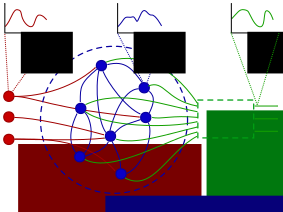
\includegraphics[width=0.6\textwidth]{figures/reservoir}
  \caption{High-level view of an echo state network RC. Each node may
    have two kinds of input connections: connections to other nodes in
    the network ($W_r$, blue), connections to the overall input
    ($W_\text{in}$, red). Each node may also have output connections
    to the overall output ($W_\text{out}$, green). Note that the
    internal connections may contain cycles.  When the RC is used to
    perform forecasting, the output on the right side is connected to
    the input on the left side, allowing the RC to run autonomously
    with no external input.}%
  \label{fig:reservoir}
\end{figure}

Put together, the dynamics of an echo state network RC are
\begin{align}
  \label{eq:esn}
  \dot{\bm{r}}(t) &= - \gamma \bm{r}(t) + \gamma \bm{f}\left( W_r\;\bm{r}(t) + W_\text{in}\;\bm{u}(t) \right), \\
  \bm{y}(t) &= W_\text{out}\;\bm{g}\left(\bm{r}(t)\right), \nonumber
\end{align}
where the vector function $\bm{f}$ is understood to mean applying the
one-dimensional activation function $f$ component-by-component. This
construction is summarized in \cref{fig:reservoir}. I will discuss
choosing the matrices $W_\text{in}$ and $W_r$, the parameter $\gamma$,
and the activation function $f$ in \cref{sec:esn-construction}.

This is the continuous-time formulation of an ESN. It is also common
to see a discrete-time formulation, which can be derived simply from
\cref{eq:esn} by the application of forward Euler
integration. Additionally, the forecasting method described in
\cref{sec:forecasting} involves a modification to the RC equation once
the RC is trained. These variations on the ESN equation are summarized
in \cref{tab:esn}.

\begin{table}
  \caption{A summary of variations of the ESN equation. The
    discrete-time formulation is the result of Euler-integrating the
    continuous-time formulation, and the forecasting variant is
    derived via the substitution described in \cref{sec:forecasting}.}
  \begin{tabular}{clrl}
    & Variation & & Equations \\
    \hline
    \rule{0pt}{4ex}
    (a) & Continuous & $\bm{\dot{r}}(t) =$ & $- \gamma \bm{r}(t) + \gamma \bm{f}\left( W_r\;\bm{r}(t) + W_\text{in}\;\bm{u}(t) \right)$ \\
    & (inference) & $\bm{y}(t) =$ & $W_\text{out}\;\bm{g}\left(\bm{r}(t)\right)$ \\
    \rule{0pt}{4ex}
    (b) & Continuous & $\bm{\dot{r}}(t) =$ & $- \gamma \bm{r}(t) + \gamma \bm{f}\left( W_r\;\bm{r}(t) + W_\text{in}\;W_\text{out}\;\bm{g}\left(\bm{r}(t)\right) \right)$ \\
    & (forecasting) & $\bm{y}(t) =$ & $W_\text{out}\;\bm{g}\left(\bm{r}(t)\right)$ \\
    \rule{0pt}{4ex}
    (c) & Discrete & $\bm{r}(t + \Delta t) =$ & $(1 - \gamma \Delta t) \bm{r}(t) + \gamma \Delta t \bm{f}\left( W_r\;\bm{r}(t) + W_\text{in}\;\bm{u}(t) \right)$ \\
    & (inference) & $\bm{y}(t + \Delta t) =$ & $W_\text{out}\;\bm{g}\left(\bm{r}(t + \Delta t)\right)$ \\
    \rule{0pt}{4ex}
    (d) & Discrete & $\bm{r}(t + \Delta t) =$ & $(1 - \gamma \Delta t) \bm{r}(t) + \gamma \Delta t \bm{f}\left( W_r\;\bm{r}(t) + W_\text{in}\;W_\text{out}\;\bm{g}\left(\bm{r}(t)\right) \right)$ \\
    & (forecasting) & $\bm{y}(t + \Delta t) =$ & $W_\text{out}\;\bm{g}\left(\bm{r}(t + \Delta t)\right)$ \\
  \end{tabular}
  \label{tab:esn}
\end{table}

% FIXME cite \gamma \Delta t = 1
The Euler integration is only an accurate representation of
\cref{eq:esn} when $\gamma \Delta t \ll 1$. However, many authors will
take $\gamma \Delta t = 1$. Although this is no longer an accurate
approximation to the continuous-time ESN in \cref{eq:esn}, these
discrete-time ESNs still function well as an RC. That the RC is not
sensitive to this kind of fundamental change in the underlying
reservoir is a hallmark of the RC method. The specific form of the
underlying reservoir is largely unimportant, except for a few
requirements to be discussed in
\cref{sec:reservoir-properties}. Indeed, the internal structure of an
ESN is determined randomly.

\section{Constructing ESNs}\label{sec:esn-construction}

The parameters $W_r$, $W_\text{in}$, $\gamma$, and $f$ in
\cref{eq:esn} must be set before the ESN construction is complete. Of
these, $\gamma$ has the most simple interpretation: it controls the
exponential decay of the value of each node in the network. If this
rate is too slow, the reservoir will not be able to react fast enough
to its input to be useful for computing the output; if this rate is
too fast, the reservoir will respond immediately to its inputs and
have no useful memory of past inputs, which may be necessary for the
RC's task. As the reservoir network may contain cycles, there is also
the possibility that a high decay rate may result in very rapid
oscillation in the network, which is undesirable if the RC's desired
output does not contain such oscillation. In practice, this decay rate
should be matched to the characteristic timescale of the output
signal, and then can be manually tuned from there if needed.

If the read-out function $\bm{g}$ is taken to be the identity
function, as is common, and the activation function $f$ is linear,
then the forecasting-mode equations in \cref{tab:esn} are completely
linear and have simple, oscillatory analytic solutions. These are
known as \emph{linear ESNs}. Linear ESNs are mathematically easy to work
with, and as a result many of the known proofs about ESNs are in the
context of linear ESNs. One of the most recent and prominent results is
discussed further in \cref{ch:nvar}.

However, because the solutions to a linear ESN in prediction mode are
so simple, it is not possible for them to reproduce the strange
attractors of chaotic systems. To do this, the activation function $f$
is used to introduce non-linearity into the equations. The most common
choice is the hyperbolic tangent, $f(x) = \tanh(x)$, and I will use this choice
in this thesis. This satisfies the non-linearity requirement, and
also ensures that each component of $\bm{r}(t)$ is bounded in $(-1,
1)$. Bounds on $\bm{r}(t)$ ensure that \cref{eq:esn} is particularly
well-behaved for numerical integrators. These bounds can also be used
to put bounds on the output $\bm{y}(t)$, which may be useful if that
output is driving a real-world system.

It is also possible to leave $f$ linear, and introduce non-linearity
into the system with $\bm{g}$. These \emph{output-layer non-linear ESNs} are
also discussed further in \cref{ch:nvar}.

The matrices $W_r$ and $W_\text{in}$, and therefore the topology and
weights of the ESN, are chosen randomly. There are many random schemes
in use, from Erd{\"{o}}s-R{\'{e}}nyi networks and small-world
networks~\cite{haluszczynski2019} to simpler cycle and line
networks.~\cite{rodan2011} The scheme I use is simple. Although this
thesis only discusses RCs simulated in software, this scheme was
designed with an eye towards hardware implementation, where the number
of inputs to each node, and the total number of connections in the
network, have an associated hardware cost.

For the internal connections $W_r$, I generate a random network where
every node has a fixed number of inputs, or \emph{in-degree}, $k$. For
each node, I select $k$ nodes in the network without replacement and
use those as inputs to the current node. Each input is assigned a
random weight drawn from a normal distribution with mean $0$ and
variance $1$. This results in a connection matrix $W_r'$ where each
row has exactly $k$ non-zero entries. Finally, I rescale the whole
matrix by
\begin{equation}
  \label{eq:setradius}
  W_r = \frac{\rho_r}{\operatorname{SR}(W_r')}\;W_r',
\end{equation}
where $\operatorname{SR}(W_r')$ is the spectral radius, or maximum
absolute eigenvalue, of the matrix $W_r'$. This scaling ensures that
$\operatorname{SR}(W_r) = \rho_r$. This parameter is used to tune the
overall scale of the recurrent weights, and therefore the importance
of recurrent connections inside the network.

For $W_\text{in}$, I randomly connect each node to each RC input in
$\bm{u}(t)$ with probability $\sigma$. The weight for each connection
is drawn randomly from a normal distribution with mean $0$ and
variance $\rho_\text{in}^2$.

Together, $\sigma$ and $\rho_\text{in}$ are enough to generate a
random instantiation of $W_\text{in}$, and $k$ and $\rho_r$ are enough
to generate a random instantiation of $W_r$. The relative scales
$\rho_r$ and $\rho_\text{in}$ determine the importance of the
recurrent and external inputs, respectively. The entire ESN construction
is then reduced to choosing these \emph{meta-parameters}, summarized in
\cref{tab:esn-metaparameters}.

\begin{table}
  \caption{Summary of echo state network meta-parameters. These
    parameters must be chosen to produce a random realization of an
    ESN-based RC.}
  \begin{tabularx}{\linewidth}{rlX}
    & Parameter & Description \\
    \hline
    \rule{0pt}{4ex}
    $N$ & Number of Nodes & the total number of nodes in the network. \\
    \rule{0pt}{4ex}
    $\gamma$ & Leak Rate & controls the exponential decay of each node. \\
    \rule{0pt}{4ex}
    $\sigma$ & Input Connectivity & the probability that any given input is connected to any given node. \\
    \rule{0pt}{4ex}
    $\rho_\text{in}$ & Input Scale & the variance of the normally-distributed input connection weights. \\
    \rule{0pt}{4ex}
    $k$ & Recurrent Connectivity & the number of input connections each node draws from other nodes in the network. \\
    \rule{0pt}{4ex}
    $\rho_r$ & Recurrent Scale & the spectral radius of $W_r$. This controls the scale of recurrent connection weights. \\
    \rule{0pt}{4ex}
    $f$ & Activation Function & the function computed at each node. This is usually $\tanh$. \\
    \rule{0pt}{4ex}
    $\bm{g}$ & Read-out Function & the output layer read-out. This is usually the identity function. \\
    \rule{0pt}{4ex}
    $\alpha$ & Ridge Parameter & regularization parameter for ridge regression \\
  \end{tabularx}
  \label{tab:esn-metaparameters}
\end{table}

\section{Properties of Good Reservoirs}\label{sec:reservoir-properties}

Which dynamic systems make for good reservoirs, and what properties
are desired in a reservoir, remains an open question. There are a
handful of known desirable properties that are used to guide reservoir
design, and in particular ESN design. Chief among these is the
\emph{fading memory property}, which states that the reservoir's
response to its input should have a vanishing dependence on the value
of that input signal in the distant past.~\cite{jaeger2001,jaeger2002}

More concretely, let $\bm{u}_1(t)$ and $\bm{u}_2(t)$ be two different
RC input signals which may differ for $t < 0$ but are otherwise
identical for $t > 0$, and let $\bm{r}_1(t)$ and $\bm{r}_2(t)$ be the
reservoir's response to these inputs. The reservoir has fading memory
if and only if $\bm{r}_1(t) \rightarrow \bm{r}_2(t)$ as $t \rightarrow \infty$.

This has many practical benefits for an RC. A reservoir with fading
memory guarantees a consistent output for a given input, regardless of
the path through state space the input takes in the distant past. This
is particularly important as running an RC often involves
resetting the internal reservoir, either in simulation or in
hardware. The fading memory property ensures that the specific initial
state of the reservoir does not matter, as long as it has a
sufficiently long warm-up time as discussed in \cref{sec:training}.

One early result for ESNs states that this fading memory property
cannot hold in an ESN when the spectral radius of the matrix $W_r$ is
greater than one~\cite{jaeger2001}, specifically because the zero
input signal $\bm{u}(t) = 0$ is unstable. Such an ESN with initial
state $\bm{r}(0) = 0$ will quickly become non-zero as soon as the
input is non-zero, and then will not return to $\bm{r} = 0$ even after
the input returns to zero.

Likewise, an ESN with $\operatorname{SR}(W_r) \ll 1$ is contracting,
and will return to $\bm{r} = 0$ rapidly with zero input. These two
considerations have combined in literature into a recommendation that
the spectral radius of $W_r$ be near, but not above,
one.~\cite{lukosevicius2012} However, both of these results are very
narrow in scope, and more recent work presented in \cref{ch:low-connectivity}
and elsewhere~\cite{pathak2017,rodan2011} show that these spectral
radius recommendations are not hard and fast rules. Nonetheless, this
history has cemented spectral radius as the standard measure of scale
for $W_r$ in ESNs.

Another desirable property of the reservoir is \emph{separability} and
\emph{continuity of response}. Similar inputs to the reservoir should produce
similar responses. This is especially important in real-world
applications, where the input to the RC is likely to be noisy. This
excludes a wide class of chaotic systems from consideration as a
reservoir, as even very small differences in two input signals would
be amplified. Likewise, a good reservoir should produce different
responses to different inputs. In the extreme case, a reservoir that
produces a constant zero regardless of input would form a very poor RC,
despite meeting the other criteria listed so far.

More recently, these requirements have been unified under the umbrella
of \emph{invertable generalized
  synchronization}~(IGS)~\cite{lu2018,lymburn2019,lu2020}, which claims that
a good reservoir is one that is synchronized to its
input. Specifically, the reservoir $\bm{r}(t)$ is in a state of
generalized synchronization with its input $\bm{u}(t)$ if there is a
function $\bm{H}$ such that, as $t \rightarrow \infty$, $\bm{r}(t)
\rightarrow \bm{H}\left(\bm{u}(t)\right)$. This already implies the
fading memory property. If $\bm{H}$ is continuous, this implies continuity of response, and if $\bm{H}$ is invertable, this implies separability. An invertable $\bm{H}$ also ensures that
\begin{equation}
  \bm{u}(t) \approx \bm{H}^{-1}\left(\bm{r}(t)\right).
\end{equation}
This is close to the form of the RC's output during forecasting in
\cref{eq:approx-output-forecast}, although there is no guarantee that
$\bm{H}^{-1}$ is linear.

The IGS approach differs from the earlier design principles in that it
considers the unified reservoir/input system together, rather than
looking for desirable properties of the reservoir
independently. Unfortunately, it yields very little actionable advice
about building a reservoir to use, and testing for the presence of IGS
in an RC computationally expensive. The quickest way to see if a
reservoir will work is still to build an RC with it, train it, and
test it. Nonetheless, this new approach unifies many older principles
in the field and is one of the most interesting avenues for future
research.

\section{Evaluating Reservoirs}

To evaluate the performance of a trained RC, it is common to use an
example testing input/output signal pair, $\bm{u}_\text{test}(t)$ and
$\bm{y}_\text{test}(t)$, that differs from the training signal. The
input $\bm{u}_\text{test}(t)$ is fed in to the trained RC, producing
the RC output $\bm{y}(t)$, which is then compared to the desired
output $\bm{y}_\text{test}(t)$. Note that the same concerns with
reservoir warm-up, as discussed in \cref{sec:training}, apply here: the
early part of the input test signal is used only to synchronize the
reservoir, and is not used in the comparison. Often, the training and
testing signals are combined such that $\bm{u}_\text{test}$ follows
directly after $\bm{u}_\text{train}$, which allows the training signal
to function as the warm-up signal for the reservoir during the testing
phase.

The most common metric for comparing the true output $\bm{y}(t)$ to
the desired output $\bm{y}_\text{test}(t)$ is to calculate the
normalized root-mean-square error (NRMSE) between them,
\begin{equation}
  \label{eq:nrmse}
  \epsilon = {\left(\sum_i\frac{\int \left| y_i(t) - y_{\text{test},i}(t) \right|^2 \;dt}{T \operatorname{Var}\left[y_{\text{test},i}(t)\right]}\right)}^{1/2},
\end{equation}
where the integral is evaluated on an interval of length $T$, and the
sum $i$ is over all components of $\bm{y}_\text{test}(t)$.  If
$\epsilon = 0$, then the two signals are identical during the interval
being evaluated, and any difference between them will result in
$\epsilon > 0$.

For RCs trained to do inference, this NRMSE is calculated across the
entire testing signal, regardless of length. However, for forecasting
this presents a problem. An RC in forecasting mode is autonomous,
after the warm-up period, and receives no ongoing external input as it
would in an inference task. The testing output may diverge quickly
from the reference system. Indeed, if the RC is trained to forecast a
chaotic system, good forecasting requires the forecast to diverge
eventually. In these situations, the testing error is calculated only
for a period of $T = 1/\lambda_\text{max}$, where $\lambda_\text{max}$
is the largest Lyapunov exponent of the system the RC is
forecasting. In this thesis, I will refer to this one Lyapunov period
error as $\epsilon_1$.

Using $\epsilon_1$ as a testing metric for forecasting RCs is common,
but still has problems.\cite{pathak2017,haluszczynski2019} The largest
issue is that the specific value of $\epsilon_1$ will depend strongly
on which specific input signal $\bm{u}_\text{test}(t)$ is used for
testing. If the input signal passes very near an unstable state of the
input system, very small errors in the RC's forecasting are amplified
dramatically. In these cases, $\epsilon_1$ is not a useful measure of
how well the RC has learned the input system. Examples of this are
given in \cref{ch:low-connectivity}.

\begin{figure}
  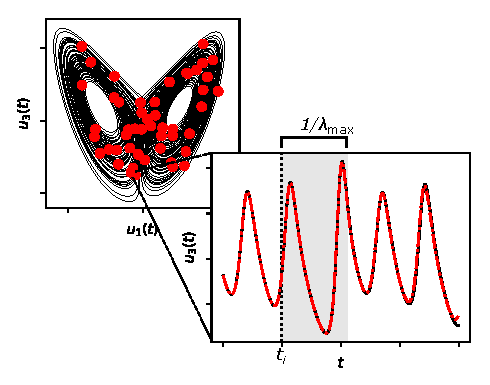
\includegraphics[width=0.6\textwidth]{figures/nrmse-avg}
  \caption{Summary of the forecasting evaluation method. I calculate
    errors $\epsilon_{1,i}$ at times $t_i$, marked on the attractor as
    red dots, and combine them into a single error
    $\tilde{\epsilon}$. Before each $t_i$ (dotted vertical line), the
    reservoir is integrated with \cref{eq:reservoir} and listening to
    the input. After $t_i$, the reservoir is integrated with
    \cref{eq:reservoir-auto}, and runs autonomously. The reservoir's
    prediction (dotted red line) must eventually diverge from the true
    system (solid black line). I calculate each $\epsilon_{1,i}$ only
    during a single Lyapunov period after forecasting begins, marked
    here in gray.}%
  \label{fig:nrmse-avg}
\end{figure}

A simple fix is to perform $m$ forecasts with many different example
inputs, calculate an $\epsilon_1$ value for each forecast, and then
combine them into one final metric
\begin{equation}
  \label{eq:nrmse-avg}
  \tilde{\epsilon} = {\left( \frac{1}{m} \sum_{i=1}^m \epsilon_{1,i}^2 \right)}^{1/2}.
\end{equation}
This method is summarized in \cref{fig:nrmse-avg}.
Using $\tilde{\epsilon}$ averages out the chance encounters with
unstable states, and as I will show in \cref{ch:low-connectivity}, is
a more reliable indicator of a forecasting RC's performance.

For forecasting, a very useful qualitative indicator of an RC's ability
to learn the input system is to use the RC in autonomous mode to
produce a very long forecast. This forecasted signal will necessarily
diverge from the true system, but both the forecast and the true
system can then be plotted side-by-side in state space. A well-trained
RC forecast will reproduce the shape of the input system's attractor,
and these plots can reveal immediate problems with the trained RC that
metrics like NRMSE sometimes mask. Still, this comparison is
completely qualitative -- it is imprecise, and not suitable to use in
an automated setting. Future research may develop a quantitative way
to measure the similarity between the RC's reconstructed attractor and
the true attractor, which would solve the problems with the current
NRMSE metric. In the meantime, visual inspection remains a useful
sanity check on the NRMSE.

\section{Summary}

Reservoir computers are a simple tool that uses an auxiliary dynamic
reservoir to transform its input. They can be trained on example data,
and that training is done very quickly using linear regression
tools. Once trained, RCs can be used in inference tasks, or in an
autonomous mode to perform system forecasting.

The RC approach is robust to the choice of reservoir system, however
the specific requirements the reservoir must have to function are
largely unknown. When an RC fails, it is difficult to know why. Recent
work on invertable generalized synchronization is an exciting path
towards learning more.

Echo state networks are a network-based reservoir choice that is easy
to simulate in software, and replicates more traditional neural
network machine learning designs. This approach uses several
meta-parameters to randomly construct the internal network. As with the
general reservoirs, there is not much concrete guidance on what values
these meta-parameters should have.

In \cref{ch:low-connectivity}, I will explore some of these
meta-parameters, and conclude that several guidelines for ESN
construction are not necessary. I will demonstrate several RCs with
very simple internal networks that nonetheless successfully replicate
the climate of a chaotic dynamic system.

\chapter{Low-Connectivity Reservoirs}\label{ch:low-connectivity}

The choice of ESN metaparameters that best fits a given task is
difficult to identify. In the absence of strong guiding rules, a
practical approach is to treat it as an optimization problem. In this
chapter, I explore using ESNs on the chaotic system forecasting task,
for the Lorenz '63 system, the R{\"{o}}ssler system, and the
double-scroll circuit system described in \cref{ch:systems}. This
exploration is guided by optimization -- by trying to discover the
metaparameters that result in the best averaged NRMSE
$\tilde{\epsilon}$ during forecasting for the given system. This
exploration leads to a surprising discovery, that even ESNs with
simple internal structure perform as well as their more complicated
siblings.

In particular, I am interested in the recurrent connectivity $k$. In
software simulations, such as those described in this thesis, the
connectivity $k$ has only a slight impact on the speed of the
simulation. However, in hardware network implementations, each
connection has an associated cost. For autonomous Boolean networks
implemented on FPGAs, every network connection is built from a long
chain of delay nodes.\cite{canaday2018} These delays often compose the
majority of the resource budget of the hardware network. Although the
results in this chapter are all software simulation, the particular
focus on the $k$ parameter is done with an eye towards hardware
implementations.

Many techniques have been used previously for ESN metaparameter
optimization, such as grid search\cite{rodan2011} and gradient
descent\cite{jaeger2007}. However, both of these approaches have
drawbacks. Grid search quickly becomes intractable when the number of
dimensions grows, and even after fixing the two functional
metaparameters $f$ and $\bm{g}$, there are 5 dimensions
left. Compounding this problem, the ESN construction is a random
process, and so the resulting measured $\tilde{\epsilon}$ for a given
set of metaparameters is a random variable. To get a meaningful
result, each set of metaparameters would need to be tested multiple
times. For even a coarse grid search, with 10 trials and 10 points per
metaparameter, this already means one million trial RCs. Gradient
descent suffers from the randomness of ESN construction as well, for
the same reasons. It is also unsuitable for use with continuous
parameters such as $k$.

The problems with random ESN construction can be mitigated by
modifying the ESN construction method outlined in
\cref{sec:esn-construction} to front-load the random choices. For
example, once the recurrent weight matrix $W_r$ has been constructed,
the parameter $\rho_r$ can be changed without any random process at
all. By cleverly factoring out the random parts of ESN construction,
it becomes possible to use methods like grid search and gradient
descent without the extra step of mulitple random trials. Ultimately,
however, this is optimizing only a single random instantiation of an
ESN, and provides little insight into how the fully random ESN will
perform.

In this chapter, I will be using Bayesian
optimization\cite{yperman2016,maat2018}, as implemented by the
\texttt{skopt} Python package\cite{skopt2018}, to explore which
metaparameters result in the lowest forecasting error
$\tilde{\epsilon}$ for the three example systems. Bayesian
optimization deals well with both noise and integer paramateres like
$k$, is more efficient than grid search,\cite{maat2018} and works well
with minimal tuning.

\section{Bayesian Optimization}

% FIXME cartoon figure for this?
Bayesian optimization is an optimization technique that finds the
minimum of an objective function $h(\bm{x})$ by repeated
evaluation. The process starts with a prior distribution of functions,
representing the algorithm's knowledge of the function $h$. As each
new point $\bm{x}$ is evaluated, the algorithm incorporates this new knowledge
and updates its prior distribution. At the start of the optimization,
points are chosen randomly. This is the exploration phase, where the
Bayesian optimizer is only gathering data to improve it's prior
distribution. After exploration, the optimizer will then evaluate
points $\bm{x}$ with the most expected improvement over the best known minimum
so far.

This algorithm has a number of drawbacks. Primarily, it is
complicated. The above summary only scratches the surface, and already
suggests a number of parameters to the optimization algorithm that can
be tuned, such as the initial prior distribution of functions. This
complication makes it difficult to directly claim that any minimum
found is the true minimum, and so I emphasize that this algorithm is
used here for exploration. I am interested in ESNs that perform well,
and what they have in common, but not in claiming any ESN as the best
performer possible. For this purpose, the unopinionated defaults of
the \texttt{skopt} package suffice.

The complexity of this optimization algorithm also manifests in run
time. After the exploration phase, calculating the next set of trial
parameters $\bm{x}$ involves minimizing an internal function
calculated from the current prior distribution. This can be quite
computationally expensive, and so Bayesian optimization is only
suitable for use when the objective function $h(\bm{x})$ is expensive
enough to justify the extra work to reduce how often it is
evaluated. This makes it a good fit for minimizing prediction error
$\tilde{\epsilon}$ as this involves building, training, and testing
an RC each time.

\begin{table}
  \caption{Range of hyperparameters searched using Bayesian optimization.}
  \begin{tabular}{lrcl}
    Parameter & min & & max \\
    \hline
    $\gamma$ & 7 & -- & 11 \\
    $\sigma$ & 0.1 & -- & 1.0 \\
    $\rho_\text{in}$ & 0.3 & -- & 1.5 \\
    $k$ & 1 & -- & 5 \\
    $\rho_r$ & 0.3 & -- & 1.5 \\
  \end{tabular}%
  \label{tab:bayes-ranges}
\end{table}

In this chapter, the Bayesian algorithm repeatedbly generates a set of
hyperparameters to test within the ranges listen in
\cref{tab:bayes-ranges}. Larger ranges would require a longer
optimization time. I selected these ranges to include values that
existing ESN design heurestics would choose, while also allowing
exploration outside those ranges without a prohibitively long runtime.

During the optimization process, I discovered that the optimizer was
often finding ESNs with $k = 1$ that perform as well as ESNs with a
higher $k$. Such networks have an interesting and simple network
structure, and also suggest other simple structures for comparison.

\section{Structure of Low-Connectivity Reservoirs}

First, networks generated with $k = 1$ often have multiple
disconnected components. For higher $k$, this is still possible but
relatively rare, as $k$ controls the number of opportunities for
components in the network to connect. Disconnected components in the
network essentially act as ESNs operating in parallel. This is an
interesting line of research,\cite{pathak2018} but not one I
investigate further here. In the interest of a more equitable
comparison between $k = 1$ networks and $k > 1$, I discard and
regenerate any networks with more than a single connected component.

\begin{figure}
  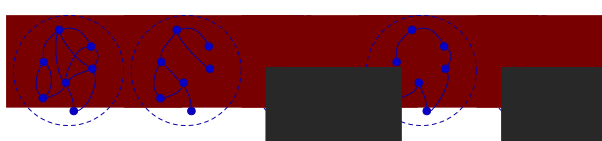
\includegraphics[width=\textwidth]{figures/topology}
  \caption{The five reservoir topologies tested. Only internal
    reservoir connections are pictured. Connections to the reservoir
    computer input, or to the output layer are not shown. (a) A
    general, fixed in-degree network, here pictured with $N=7$ and
    $k=2$. (b) A $k=1$ network with a single connected component. (c)
    A $k=1$ network with the single cycle cut at an arbitrary
    point. (d) A \emph{simple cycle reservoir}. (e) A \emph{delay line
      reservoir}.}%
  \label{fig:topology}
\end{figure}

A $k = 1$ network with only a single connected component must also
contain only a single directed cycle. Starting from any node in the
network and working backwards through the single input connection each
node must have will always lead to a single directed cycle, and it is
not possible for two such cycles to exist in the network unless they
are disconnected from each other. This severely limits how recurrence
can occur inside a $k = 1$ network compared to higher-$k$
networks. Every node in a $k = 1$ network is either part of this core
cycle, or part of a directed tree branching off from this cycle, as
depicted in \cref{fig:topology}~(b).

Inspired by the high performance of this simple structure, I also
investigate $k = 1$ networks when the single cycle is cut at a random
point. This turns the entire network into a tree, as in
\cref{fig:topology}~(c).

Finally, I also investigate reservoir networks that consist entirely
of a cycle or a ring with identical weights with no attached tree
structure, depicted in \cref{fig:topology}~(d), and networks with a
single line of nodes (a cycle that has been cut), in
\cref{fig:topology}~(e). These choices were inspired by the $k = 1$
networks, but have also been researched previously and are known as
\emph{simple cycle reservoirs} and \emph{delay line reservoirs},
respectively.\cite{rodan2011}

\section{RC Symmetries and their Consequences}

An ESN in autonomous forecast mode, described by \cref{tab:esn}~(b),
has an inversion symmetry about the origin. That is, if $\bm{r}(t)$ is
a solution to this equation, so is $-\bm{r}(t)$. For an output layer
with an identity read-out function $\bm{g}$, this means that if
$\bm{y}(t)$ is a possible output of the trained RC, then so is
$-\bm{y}(t)$. If the underlying system the RC was trained to forecast
also exhibits this symmetry, this is not a problem. In fact, designing
the internal reservoir to match symmetries with the input system can
dramatically improve RC performance\cite{barbosa2021}.

However, if the input system does not have this symmetry, this can be
an issue. If at any time the autonomous forecast strays near $\bm{r} =
0$, the solution can hop over the symmetry to the other side, and
begin producing an output $\bm{y}(t)$ that is flipped through the
origin. This problem is exacerbated if the input signal $\bm{u}(t)$ is
normalized to have mean zero, a common practice.

This problem was identified early, and a common fix\cite{pathak2017,herteux2020}
is to use a non-linear read-out function
\begin{equation}
  g_i(\bm{r}) = \begin{cases}
    r_i & \text{if } i \leq N / 2, \\
    r_i(t)^2 & \text{if } i > N / 2.
  \end{cases}
  \label{eq:esn-break-sym}
\end{equation}
This squares half of the node values before being passed
to the output layer, and breaks the inversion symmetry in the ESN
equation while keeping the number of features accessible to the output
layer the same.

%score: 0.08873905001779689
%score-1: 0.007877037205449461
\begin{figure}
  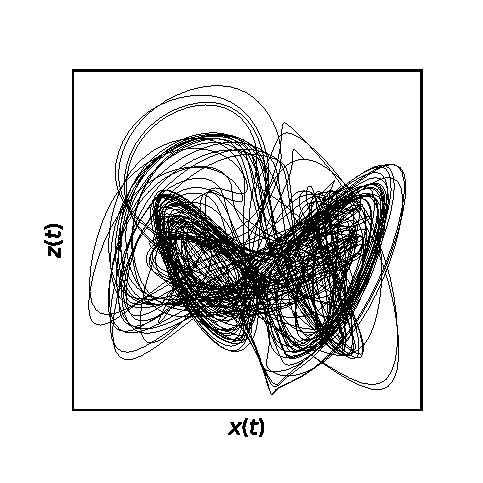
\includegraphics[width=0.5\textwidth]{figures/lorenz-symmetry}
  \caption{The forecasted attractor from an ESN trained on the Lorenz
    '63 system, with identity read-out, in the $x$/$z$ plane. Compare
    against \cref{fig:lorenz}, and note the two deformed images of the
    butterfly attractor on top of each other, with one flipped along
    the $z$ axis.}
  \label{fig:lorenz-symmetry}
\end{figure}

This problem can be difficult to diagnose if the input system has a
partial inversion symmetry. For example, the Lorenz '63 system in
\cref{eq:lorenz} has an $(x, y) \rightarrow (-x, -y)$ symmetry, and so the
complete inversion of the Lorenz attractor looks exactly the same as a
flip along the $z$ axis. This is misleading, as the problem has
nothing to do with the Lorenz $z$ variable specifically, and this
confusion prevented a full understanding of the problem until
recently.\cite{herteux2020} \cref{fig:lorenz-symmetry} provides an
example of the forecasting failure characteristic to the identity
read-out function.

For consistency, I use this \emph{quadratic read-out} for all three
example input systems, even if the inversion symmetry exists in the
input system as it does for the double-scroll circuit.

\section{Training, Forecasting, and Evaluation}
% use mean 0 variance 1 signals from systems ...
% length of time periods
% use cross-validation for alpha
% discussion of \tilde{\epsilon} vs \epsilon

\section{Results}
% detailed results for lorenz, violin plots, attractors
% for other systems

\section{Cross-task Performance}
% optimized Lorenz used on double-scroll

\section{Conclusion}
% optimization is useful, and can yield surprising results
% \tilde{\epsilon} is good
% rho_r = 0, k=1 are useful (weird!)
% but: they are rarer. This might be useful
% NARX note: also look forward to next chapter. what unifies these?
% line reservoir is almost just some time delay taps
% can this generalize to many tasks? can it make hardware simpler?

\chapter{RCs without Reservoirs: Non-linear Vector Auto-regressions}\label{ch:nvar}

In 2021, Erik Bollt proved~\cite{bollt2021} that a completely linear
ESN is mathematically equivalent to an existing tool known as a \emph{vector
auto-regression}, or VAR. He subsequently proved that an ESN with a
quadratic output non-linearity is likewise equivalent to a
\emph{non-linear VAR}, or NVAR.

In this chapter, I provide a brief outline of this equivalence proof,
beginning with a discussion of the behavior of fully linear ESNs as
well as their drawbacks. Later, I describe the VAR and NVAR
methods. This provides background information and motivation for the
original work presented in \cref{ch:nvar-application}.

Although output-non-linear ESNs and NVARs are mathematically
equivalent, the conditions of their equivalence raise some practical
concerns when it comes to implementation. In this chapter will discuss
these concerns, as well as the relative merits of the ESN and NVAR
approaches. In addition, I discuss how the NVAR approach benefits from
reinterpretation within the RC framework.

In \cref{ch:nvar-application} I will build on the information provided
here to demonstrate the NVAR approach in practical applications, and
quell these concerns about the applicability of Bollt's proof.

\section{Solutions to Linear ESNs}

\subsection{Prediction}

A fully linear ESN, with both the activation function $f$ and the
read-out function $\bm{g}$ set to the identity function, has very
simple solutions. 
As an example, I will take the discrete-time linear
ESN equation in prediction mode from \cref{tab:esn}~(d),
\begin{align}
  \bm{r}(t + \Delta t) &= (1 - \gamma \Delta t) \bm{r}(t) + \gamma \Delta t \left( W_r\;\bm{r}(t) + W_\text{in}\;W_\text{out}\;\bm{r}(t)\right), \label{eq:nvar-esn-forecast} \\
  \bm{y}(t+\Delta t) &= W_\text{out}\;\bm{r}(t+\Delta t).
\end{align}
The linear coefficients of $\bm{r}(t)$ can be collected into a single matrix
\begin{equation}
  W \equiv (1 - \gamma \Delta t) I + \gamma \Delta t \left( W_r + W_\text{in}\;W_\text{out}\right),
\end{equation}
simplifying the \cref{eq:nvar-esn-forecast} to
\begin{equation}
  \bm{r}(t + \Delta t) = W\;\bm{r}(t).
\end{equation}
Almost all square matrices of complex numbers are diagonalizable. If
$W$ is an $N \times N$ matrix, diagonalizing $W$ yields $N$
independent time evolution equations $r_i(t + \Delta t) = w_i\;
r_i(t)$ where $w_i$ may be complex. Solutions to this equation are very simple,
\begin{equation}
  r_i(k \Delta t) = w_i^k\; r_i(0).
\end{equation}

This means the dynamics of the ESN amount to discrete-time complex
waves, possibly with an exponential growth or decay over time. This is
all the RC output layer has to draw from to construct the output
$\bm{y}(t)$. For the forecasting task, a sum of sine waves of
different frequencies can perform adequately well for short-term
prediction~\cite{bollt2021}, as this effectively amounts to a discrete Fourier
approximation. However, for long term attractor reconstruction and the
reproduction of global properties of the input system, this linear ESN
\emph{must} eventually fail on anything but the simplest input
system. The most direct demonstration of this failure is that this
linear ESN cannot predict any fixed point of the input system except
$\bm{y}(t) = 0$.

To have any hope of reconstructing the underlying system attractor, as
demonstrated with ESNs in \cref{ch:low-connectivity}, an ESN must have some non-linear component, either in the
activation function $f$ or the read-out function
$\bm{g}$. Still, a completely linear ESN is mathematically easy to
work with, and indeed the RC/NVAR equivalence proof begins by looking
at the behavior of a discrete-time linear ESN in inference mode.

\subsection{Inference}

For ESNs in inference mode, from \cref{tab:esn}~(c),
\begin{align}
  \bm{r}(t + \Delta t) &= (1 - \gamma \Delta t) \bm{r}(t) + \gamma \Delta t \left( W_r\;\bm{r}(t) + W_\text{in}\;\bm{u}(t) \right), \label{eq:nvar-esn} \\
  \bm{y}(t+\Delta t) &= W_\text{out}\;\bm{r}(t+\Delta t). \label{eq:nvar-esn-output}
\end{align}
The coefficients of $\bm{r}(t)$ and $\bm{u}(t)$ can be collected into two matrices,
\begin{align}
  A &\equiv (1 - \gamma \Delta t) I + \gamma \Delta t W_r, \\
  B &\equiv \gamma \Delta t W_\text{in}.
\end{align}
\Cref{eq:nvar-esn} then simplifies to
\begin{equation}
  \bm{r}(t + \Delta t) = B\;\bm{u}(t) + A\;\bm{r}(t).
\end{equation}
This equation is recursive; expanding it out into the past yields
\begin{align}
  \bm{r}(t + \Delta t) &= B\;\bm{u}(t) + AB\;\bm{u}(t - \Delta t) + A^2\;\bm{r}(t), \\
  \bm{r}(t + \Delta t) &= \sum_{j = 0}^\infty A^j B \bm{u}(t - j \Delta t). \label{eq:esn-var-mat}
\end{align}

\Cref{eq:esn-var-mat} states that the value of $\bm{r}(t + \Delta t)$
is constructed from a linear combination of time-delay taps of the
input $\bm{u}(t)$, extending infinitely into the past.  In combination
with \cref{eq:nvar-esn-output}, this means the overall output
$\bm{y}(t)$ is a linear combination of time-delay taps of the input
$\bm{u}(t)$.  This is known as a vector auto-regression.

\section{Linear Vector Auto-regressions (VARs)}

In most cases, the term \emph{vector auto-regression} specifically
means a method of producing an output $\bm{y}(t)$ from a linear
combination of past outputs. However, I will generalize this slightly
in order to better mirror the reservoir computer model introduced in
\cref{ch:reservoir-computing}.

In this thesis, a vector auto-regression (VAR) is a method of
transforming a discrete-time input signal $\bm{u}(t)$ into a
discrete-time output signal $\bm{y}(t)$ from a linear combination of
time-delay taps. Given a list of tap delays $\tau_i$, I construct
a tap vector $\bm{v}(t)$ via
\begin{equation}
  \label{eq:var-v}
  \bm{v}(t + \Delta t) = \bm{u}(t - \tau_0 \Delta t) \oplus \bm{u}(t - \tau_1 \Delta t) \oplus \cdots \oplus \bm{u}(t - \tau_{q-1} \Delta t)
\end{equation}
where the operator $\oplus$ is understood to mean vector
concatenation. That is, if the input $\bm{u}(t)$ has dimension $d$,
and if there are $q$ taps, then the vector $\bm{v}(t)$ has dimension
$dq$. Most commonly, $\tau_0 = 0$, which ensures that the VAR has access to the most recent information from $\bm{u}(t)$ when producing an output.

\begin{figure}
  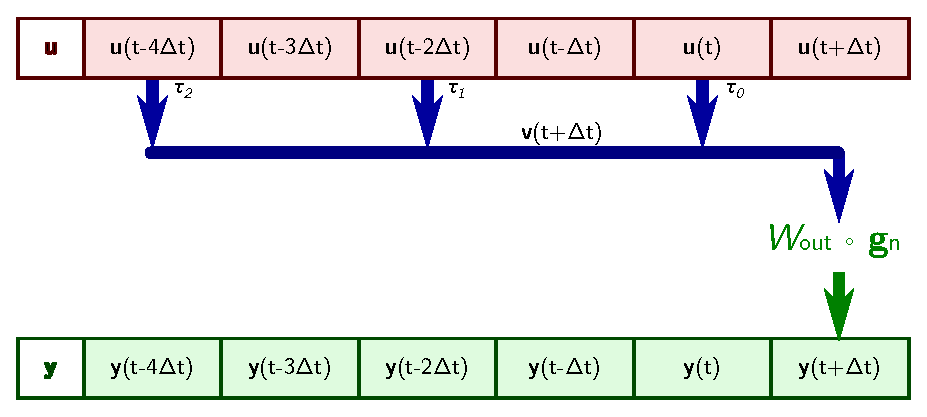
\includegraphics{figures/var-infer}
    \caption{Summary of the (N)VAR method. Many time-delay taps $\tau_i$
    of the discrete-time signal $\bm{u}(t)$ (top, red) are concatenated into the tap
    vector $\bm{v}(t)$ (middle, blue). Here, there are three taps
    $\tau_0=0$, $\tau_1=2$, and $\tau_2=4$. These taps are then passed
    through a possibly nonlinear function $\bm{g}_\text{n}$ and
    combined linearly by the output matrix $W_\text{out}$ to produce
    the next value of the (N)VAR's output $\bm{y}(t)$ (bottom,
    green). For a linear VAR, $\bm{g}_\text{n}$ is the identity
    function. To transform a whole time series input, this (N)VAR process
    slides along the time axis from left to right.}
  \label{fig:var-infer}
\end{figure}

The output of the VAR is a linear transformation of this tap vector,
\begin{equation}
  \label{eq:var-y}
  \bm{y}(t + \Delta t) = W_\text{out}\;\bm{g}_\text{n}\left(\bm{v}(t + \Delta t)\right),
\end{equation}
where $\bm{g}_\text{n}$ is the identity function. If $\bm{g}_\text{n}$
is instead chosen to be non-linear, this results in a non-linear VAR
which I discuss in \cref{sec:nvar}.

This transformation process, from input to output, is summarized in
\cref{fig:var-infer}. Note the similarity to the RC method: the input
signal $\bm{u}(t)$ drives an internal state $\bm{v}(t)$ / $\bm{r}(t)$,
which is then linearly transformed into the output
$\bm{y}(t)$. However, the internal state $\bm{v}(t)$ of the VAR is
much simpler than that of most reservoirs, since it is constructed
directly from the input.

\subsection{Training and Testing}

Once the taps $\tau_i$ are selected, the VAR can be trained in much
the same way as an RC. The VAR is fed an example input
$\bm{u}_\text{train}(t)$, which produces an example tap vector
$\bm{v}_\text{train}(t)$ via \cref{eq:var-v}. Finally, a $W_\text{out}$
that best maps this $\bm{v}_\text{train}(t)$ onto the example output
$\bm{y}_\text{train}(t)$ can be found via ridge regression, exactly as
in the RC case.

VARs can also be used for forecasting as well. Analogously to the RC
case, the VAR used for forecasting can be trained to reproduce the
example input as its output. Since the VAR output $\bm{y}(t + \Delta
t)$ depends only on $\bm{u}(t)$ at time $t$ and earlier, this amounts
to one step ahead prediction. Once trained, the VAR can do autonomous
prediction by replacing the input $\bm{u}(t)$ with the output
$\bm{y}(t)$ in \cref{eq:var-v}.

For practical reasons, in this thesis forecasting VARs have a modified
output equation
\begin{equation}
  \bm{y}(t + \Delta t) = \bm{u}(t) + W_\text{out}\;\bm{g}_\text{n}\left(\bm{v}(t + \Delta t)\right).
\end{equation}
This effectively changes the VAR from one step ahead prediction to
predicting the difference between the last value of the signal and the
next, in analogy to a discrete time integrator. Without this change,
the components of $W_\text{out}$ corresponding to $\bm{u}(t)$ would be
larger than the others. Since the ridge regression used to find
$W_\text{out}$ has a single regularization parameter $\alpha$, it
works best when all components of $W_\text{out}$ have about the same
expected scale.

Once trained, either as a signal transformation or for prediction, a
VAR can be tested in the same ways as an RC. For signal
transformations, the VAR output is compared to the true signal,
yielding a NRMSE $\epsilon$. For prediction, the VAR can be used to
generate multiple predictions for a single Lyapunov time, and the
NRMSE $\epsilon_1$ from these predictions is combined into an average
error $\tilde{\epsilon}$.

\subsection{Comparing VARs to ESNs}

Working with a VAR, by training it and using it, is very similar to
working with an RC. The most important difference is that using a VAR
completely sidesteps the issue of choosing an internal
reservoir. Building an ESN reservoir is a complicated process that
starts with the meta-parameters listed in \cref{tab:esn-metaparameters}
and ends with a random realization of a network, usually of 100 nodes
or more. In contrast, building a VAR amounts to selecting which taps
$\tau_i$ to use, and how many.

By describing the VAR method within the reservoir computing framework,
there are a few benefits to the VAR method as well. Previous work with
VARs has trained the $W_\text{out}$ matrix with least squares, while
work in the RC field has long used ridge regression as a way to reduce
overfitting and encourage generalization. In addition, VARs benefit
from the more sophisticated forecasting evaluation methods, such as
$\tilde{\epsilon}$, developed for use with RCs.

However, the linear ESN solution in \cref{eq:esn-var-mat} is only
completely equivalent to a VAR with an infinite number of time delay
taps. VARs with a finite number of taps $q$ will approximate a VAR
with infinite taps under the right conditions as $q \rightarrow
\infty$~\cite{bollt2021}, but if VARs are to be used as a replacement
for RCs, it is critical to know how good this approximation is in
practice. If a VAR requires thousands of taps to work, it may still
be simpler just to use an ESN.

Finally, these linear VARs suffer from the same drawbacks as the
linear ESN. Any practical replacement for a full, non-linear ESN would have to
reproduce the attractors of the systems they are trained on, as in
\cref{ch:low-connectivity}, and to do that, they need a non-linearity.

\section{Non-linear Vector Autoregressions (NVARs)}\label{sec:nvar}

The ESN model has two possible sources of non-linearity: the
activation function $f$ and the read-out function $\bm{g}$. Most
commonly, including in \cref{ch:low-connectivity}, $f =
\tanh$. However, a non-linear $f$ is mathematically difficult to work
with, as it lies in the middle of the ESNs internal state equation. In
contrast, the read-out function $\bm{g}$ sits only on the output
layer. Consider the linear ESN described in
\cref{eq:esn-var-mat} modified to have a non-linear read-out function
\begin{equation}
  g_i(\bm{r}) = \begin{cases}
    r_i & \text{if } i \leq N, \\
    r_{i - N}^2 & \text{if } N < i \leq 2N.
  \end{cases}
  \label{eq:esn-quadratic-out}
\end{equation}
where $N$ is the number of nodes in the ESN.  That is,
$\bm{g}(\bm{r})$ contains all of the node values, as well as the
square of all the node values. This is similar to the read-out
function used in \cref{ch:low-connectivity}, except that it makes no
attempt to keep the dimension of $\bm{g}(\bm{r})$ the same as the dimension of $\bm{r}$. By
\cref{eq:esn-var-mat}, each node value is a linear combination of
time-delay taps of $\bm{u}(t)$, and so the square of a node value will
contain only quadratic terms of the form $u_i(t-j\Delta
t)u_k(t-l\Delta t)$.

Putting this together, the ESNs output $\bm{y}(t)$ can written in
terms of the time-delay tap vector $\bm{v}(t)$ in \cref{eq:var-v},
using an infinite number of taps $\tau_i = i$,
\begin{equation}
  \bm{y}(t + \Delta t) = W_\text{out}\;\bm{g}_\text{n}\left(\bm{v}(t + \Delta t)\right).
\end{equation}
The non-linear function $\bm{g}_\text{n}(\bm{v})$ has all
components of $\bm{v}$ as well as all quadratic pairs of those components,
\begin{equation}
  \label{eq:quadratic-nvar}
  \bm{g}_\text{n}(\bm{v}) = \bm{v} \oplus \ceil{\bm{v} \otimes \bm{v}}.
\end{equation}
Here, the operator $\otimes$ denotes the outer product, and $\ceil{X}$
denotes the a flattened vector that contains the upper-triangular
components of $X$. For example, $\ceil{\bm{v} \otimes \bm{v}}$ is a
vector that contains as components all unique terms of the form $v_i
v_j$.

This construction, a VAR that wraps the delay tap vector in a
non-linear function $\bm{g}_\text{N}$ before the building the linear
combination for the output, is known as a non-linear VAR (NVAR). This
concludes a sketch of Bollt's proof that a linear ESN with quadratic
read-out is mathematically equivalent to an NVAR with infinite
taps~\cite{bollt2021}. Because the read-out function appears only on
the output, it is not difficult to change the nature of the non-linear
read-out $\bm{g}$ in an ESN and derive the corresponding NVAR $\bm{g}_\text{n}$,
and therefore this proof generalizes easily to read-out functions that are more
complicated than quadratic.

It is important to note at this point that the ESN's output weights
$W_\text{out}$ and read-out $\bm{g}$ are \emph{not} the same as the
equivalent NVAR's output weights $W_\text{out}$ and non-linearity
$\bm{g}_\text{out}$. In this example, the ESN's $\bm{g}$ produces node values and squares of node
values, while the NVAR's $\bm{g}_\text{n}$ produces all linear and
quadratic terms it is possible to construct from the tap vector
$\bm{v}$. The NVAR has quadratic terms that mix both the dimensions of the input $\bm{u}(t)$ as well as mix the tap delays $\tau_i$. In a practical application with a finite tap vector, this
means that if $\bm{v}$ has $q$ taps, then $\bm{g}_\text{n}$ will have
$q + q(q+1)/2$ components. This quadratic dependence on $q$ can
rapidly cause the computational cost of the ridge regression to find $W_\text{out}$ to be very
expensive.

Putting all the pieces together, the NVAR method for transforming an
input $\bm{u}(t)$ into an output $\bm{y}(t)$ is described by
\begin{align}
  \label{eq:nvar}
  \bm{v}(t + \Delta t) &= \bm{u}(t - \tau_0 \Delta t) \oplus \bm{u}(t - \tau_1 \Delta t) \oplus \cdots \oplus \bm{u}(t - \tau_{k-1} \Delta t), \\
  \label{eq:nvar-out}
  \bm{y}(t + \Delta t) &= W_\text{out}\;\bm{g}_\text{n}\left(\bm{v}(t + \Delta t)\right).
\end{align}
For forecasting tasks, the output \cref{eq:nvar-out} is replaced with
\begin{equation}
  \label{eq:nvar-out-forecast}
  \bm{y}(t + \Delta t) = \bm{u}(t) + W_\text{out}\;\bm{g}_\text{n}\left(\bm{v}(t + \Delta t)\right).
\end{equation}

Simply by wrapping the tap vector $\bm{v}$ in a non-linear function
before the output, the NVAR now has the non-linearity required to have
any hope of reproducing attractors as well as the non-linear ESNs, and
in \cref{ch:nvar-application} I will demonstrate that NVARs perform
quite well in this role.

\section{Practical Considerations}

The above sketch of Bollt's proof demonstrates that a linear ESN with non-linear
readout is equivalent to an NVAR with an infinite number of taps. In
practice, though, this method can only be implemented with a finite
number of taps. If an NVAR implementation requires thousands of taps
to work, it is not a realistic replacement for the ESN method.

The number of taps $q$ used is also relevant for the quadratic
$\bm{g}_\text{n}$ described in \cref{eq:quadratic-nvar}. The output
dimension of this function, $q + q(q + 1)/2$, is also one of the
dimensions of the output matrix $W_\text{out}$. As this dimension
grows, so does the time required to perform ridge regression. This
quadratic dependence on $q$ also emphasizes the need to keep the
number of taps low.

On top of this, a quadratic output may not be enough. If a quadratic
NVAR is trained to do forecasting on a system with total inversion
symmetry $\bm{u}(t) \rightarrow -\bm{u}(t)$, the quadratic terms in
the output cannot meaningfully contribute. This reduces the NVAR to a
linear VAR, with all the forecasting problems that entails. To use an
NVAR on such a system, the non-linear function $\bm{g}_\text{n}$ must
be expanded to include higher-order terms. This can be done by
constructing an ESN and calculating the equivalent NVAR form, but it
can also be done more directly by simply adding higher-order monomial terms to
$\bm{g}_\text{n}$. I will explore this in
\cref{ch:nvar-application}. However, this further emphasizes the
requirement for a small number of taps, as the number of terms of
order $n$ grows as $q^n$.

\begin{table}
  \caption{Summary of NVAR parameters. Compared to the ESN approach in
    \cref{tab:esn-metaparameters}, the NVAR method is much simpler.}
  \begin{tabularx}{\linewidth}{rlX}
    & Parameter & Description \\
    \hline
    \rule{0pt}{4ex}
    $\tau_i$ & Tap Delays & the placement of time-delay taps \\
    \rule{0pt}{4ex}
    $\bm{g}_\text{n}$ & Read-out Function & the non-linearity on the output layer \\
    \rule{0pt}{4ex}
    $\Delta t$ & Time Step & the discrete time step of both the input $\bm{u}(t)$ and the NVAR itself \\
    \rule{0pt}{4ex}
    $\alpha$ & Ridge Parameter & regularization parameter for ridge regression \\
  \end{tabularx}
  \label{tab:nvar-parameters}
\end{table}

If these challenges can be overcome, NVARs are an extremely appealing
replacement for the ESN approach. ESNs are complicated random networks
with many poorly-understood meta-parameters. In contrast, NVARs have
only four total parameters, listed in \cref{tab:nvar-parameters}.  In
addition to being a smaller set of parameters, these parameters are
simply much more interpretable. It is not straightforward to imagine
what changing the input connectivity of an ESN will do to performance,
but changing the taps $\tau_i$ has a direct effect on what information
is available to the NVAR.

\section{Summary}

VARs and NVARs are, like RCs, a method of transforming an input signal
into an output signal. They operate on linear combinations of
time-delay taps of the input. In many ways, their construction and use
mirrors that of an RC, except that there is no internal dynamic
reservoir system. This sidesteps a whole host of questions and
decisions relating to reservoir construction, and dramatically
simplifies the implementation of VARs and NVARs. However, despite this
simplicity, they are now known to be mathematically equivalent to an
ouput layer non-linear ESN.

NVARs are an established method, and this equivalence opens the door
to cross-talk between the NVAR and RC communities. On the RC side,
researchers gain a dramatically simpler implementation that is known
to be equivalent, and also gain a chance to apply lessons learned in
the RC world to the NVAR method. The NVAR approach benefits from the
use of ridge regression, long used in the RC field, instead of other
linear fitting methods.  It also benefits from improvements to
evaluation, such as $\tilde{\epsilon}$, and opens the door to using
NVARs on traditional RC problems. However, some questions still
remain -- most notably, how many time-delay taps are practically
necessary, and how complicated a non-linear function will most tasks
need?

If these questions are resolved, the NVAR approach is an extremely
attractive alternative to the ESN approach. NVARs do not rely on
random construction, are simple to implement, and have only a few
parameters with direct interpretations. If NVARs work well, it becomes
difficult to recommend ESNs and the complications they entail.

In the next chapter, I will apply the NVAR method to the traditional
RC tasks of system state inference and chaotic system forecasting. In
the process, I will resolve these remaining questions, and demonstrate
that NVARs are a practical and very simple replacement for traditional
ESN approaches.

\chapter{NVARs in Practice}\label{ch:nvar-application}


\chapter{Conclusion}\label{ch:conclusion}

In this dissertation, I challenge common RC design rules, and
demonstrate increasingly simple RCs that break these rules and still
perform well.

In \cref{ch:low-connectivity}, I demonstrate ESN-based RCs with five
classes of simple internal connectivity that all perform well on the
system forecasting task. Despite the fact that recurrence is a common
requirement in ESN design, two of these classes of connectivity have
\emph{no recurrence}, but continue to perform well. A network with only a
single internal cycle, or no cycles at all, can perform as well as a
network with many recurrent cycles. These simpler reservoir structures
may benefit hardware-based RCs, where every internal connection has an
associated cost.

This work reveals some new lines of possible future
research. Primarily, the $\tilde{\epsilon}$ metric is a more valuable
measure than $\epsilon_1$ of how well the ESN reproduces the climate
of the system, but ultimately still fails to measure attractor
similarity directly. The development of such a metric would be very
important to the field, as it begins to consider how well an RC
reproduces climate in addition to short-term forecasting.

One of the simple connectivity classes I explore is a simple line
network. The fact that this line network can perform as well as a
full-connectivity network indicates that perhaps the reservoir's role
is to produce a variety of time delays for the RC output layer to draw
on. In \cref{ch:nvar}, I summarize the NVAR method, which parallels
the RC method but instead takes time-delay taps of the input directly
rather than relying on a reservoir. I also sketch a new proof in the
field of reservoir computing that shows a certain type of
output-nonlinear ESN is equivalent to an infinite-tap NVAR.

In \cref{ch:nvar-application} I build on this proof with my
collaborators to implement NVARs that solve the traditional RC tasks
of system state inference and system forecasting. I show
that the NVAR can solve these tasks with only a few, finite taps, and
that the specific nonlinearity used in the proof can be modified an
extended in obvious ways to expand the number of problems it can
solve. This opens the door to an entire expanding tree of interesting
research. Now any task previously solved in an RC context can be
attempted in an NVAR context, and the success or failure of the NVAR
at solving a given problem will contribute meaningfully to both the
NVAR and RC fields.

Applying the NVAR approach to Mackey-Glass system forecasting reveals
possibly the most important avenue for future research. Cubic terms
are not sufficient for all problems, but adding higher-order monomials
directly to the NVAR leads to an exponential explosion in training
time. Future research will need to resolve this by including these
higher-order terms without exhaustively including all monomials, and
may possibly make use of nonlinear functions with infinite power
series.

The NVAR is a reservoir computer pruned down to its most essential
components, and now that I know it is possible build a high-performance reservoir computer
without a reservoir \emph{at all}, I am excited to see what new
directions the RC field moves towards.


\backmatter
%\nocite{*}
\bibliography{thesis}

\appendix
\chapter{Example Systems}\label{ch:systems}

Reservoir computers are most useful as tools for answering questions
about dynamic systems, such as state inference and
forecasting. Throughout this dissertation, I use many small chaotic systems
for example RC tasks. For reference, they are included here.

\section{Lorenz '63}\label{sec:lorenz}

\begin{figure}
  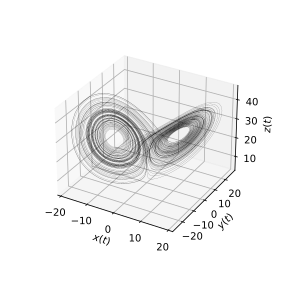
\includegraphics[width=0.7\textwidth]{figures/lorenz-3d}
  \caption{The true Lorenz attractor, produced by integrating \cref{eq:lorenz}.}%
  \label{fig:lorenz-3d}
\end{figure}

\begin{figure}
  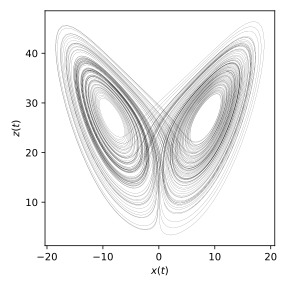
\includegraphics[width=0.6\textwidth]{figures/lorenz}
  \caption{The true Lorenz attractor projected on to the $x$/$z$ plane.}%
  \label{fig:lorenz}
\end{figure}

The Lorenz '63 chaotic system is described by
\begin{equation}
  \begin{aligned}
    \dot{x} &= \sigma \left(y - x\right), \\
    \dot{y} &= x \left(\rho - z\right) - y, \\
    \dot{z} &= x\,y - \beta z,
  \end{aligned}
  \label{eq:lorenz}
\end{equation}
with standard parameters $\sigma = 10$, $\rho = 28$, and $\beta = 8/3$~\cite{lorenz1963}. The attractor of this
system in \cref{fig:lorenz-3d} can be visualized easily in two dimensions by projecting the
three-dimensional trajectory of the system onto a plane. I show the
attractor in the $x$/$z$ plane in \cref{fig:lorenz}, and I use this projection throughout this dissertation whenever I compare ESN or NVAR output to the true Lorenz attractor.

\section{R{\"{o}}ssler}\label{sec:rossler}

\begin{figure}
  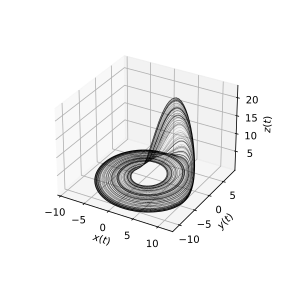
\includegraphics[width=0.6\textwidth]{figures/rossler-3d}
  \caption{The true R{\"{o}}ssler attractor, produced by integrating \cref{eq:rossler}.}%
  \label{fig:rossler-3d}
\end{figure}

%\begin{figure}
%  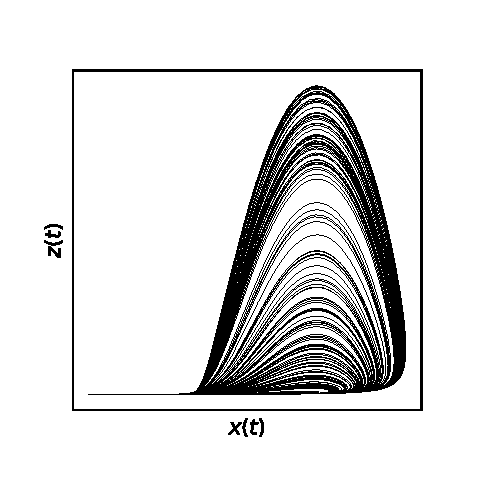
\includegraphics[width=0.6\textwidth]{figures/rossler}
%  \caption{The true R{\"{o}}ssler attractor projected on to the $x$/$z$ plane.}
%  \label{fig:rossler}
%\end{figure}

The R{\"{o}}ssler system is described by
\begin{equation}
  \begin{aligned}
    \dot{x} &= - y - z, \\
    \dot{y} &= x + a y, \\
    \dot{z} &= b + z (x - c),
  \end{aligned}
  \label{eq:rossler}
\end{equation}
with standard parameters $a = 0.2$, $b = 0.2$, $c =
5.7$~\cite{rossler1976}. The attractor of this system is visualized in
\cref{fig:rossler-3d}.

The $z$ component of this system mostly stays near zero, with rare
positive spikes. This makes prediction with an ESN difficult. To make
this component of the system more suitable for ESN prediction, I use
$\log z$ instead for both ESN input and prediction output.

\section{Double-Scroll}\label{sec:dscroll}

\begin{figure}
  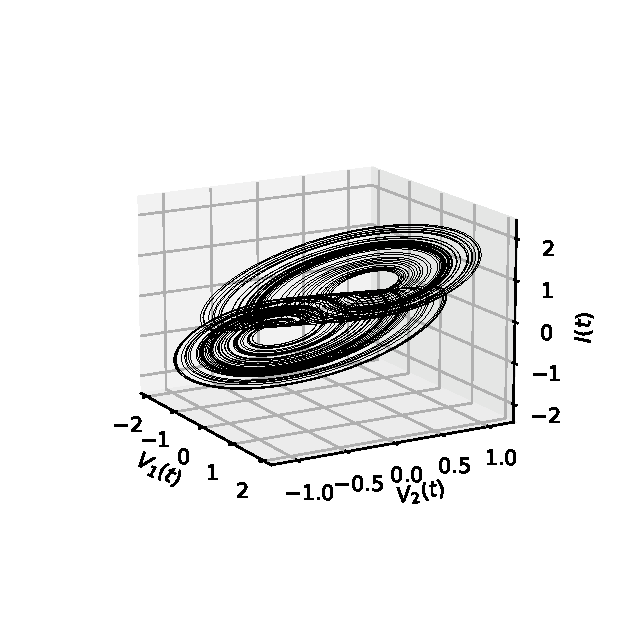
\includegraphics[width=0.7\textwidth]{figures/dscroll-3d}
  \caption{The true double-scroll circuit attractor, produced by integrating \cref{eq:dscroll}.}%
  \label{fig:dscroll-3d}
\end{figure}

\begin{figure}
  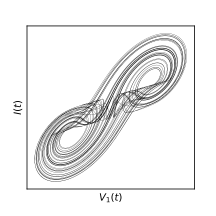
\includegraphics[width=0.6\textwidth]{figures/dscroll}
  \caption{The true double-scroll circuit attractor projected on to the $V_1$/$I$ plane.}%
  \label{fig:dscroll}
\end{figure}

The double-scroll chaotic circuit is described by the dimensionless equations
\begin{equation}
 \begin{aligned}
   \dot{V_1} &= \frac{V_1}{R_1} - \frac{V_1 - V_2}{R_2} - 2 I_r \sinh\left(\alpha(V_1 - V_2)\right), \\
   \dot{V_2} &= \frac{V_1 - V_2}{R_2} + 2 I_r \sinh\left(\alpha(V_1 - V_2)\right) - I, \\
   \dot{I} &= V_2 - R_4 I,
 \end{aligned}
 \label{eq:dscroll}
\end{equation}
with parameters $R_1 = 1.2$, $R_2 = 3.44$, $R_4 = 0.193$, $I_r = 2.25
\times 10^{-5}$, and $\alpha = 11.6$~\cite{gauthier1996}. The
attractor of this system is depicted in \cref{fig:dscroll-3d}. As
with the Lorenz system, for comparison purposes I will use a
projection of the attractor on to the $V_1$/$I$ plane, depicted in
\cref{fig:dscroll}.

\section{Mackey-Glass}\label{sec:mackey-glass}

\begin{figure}
  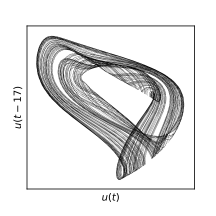
\includegraphics[width=0.6\textwidth]{figures/mackey-glass}
  \caption{The true Mackey-Glass attractor represented as a time delay embedding using $\tau$ as the delay, produced by integrating \cref{eq:mackey-glass}.}%
  \label{fig:mackey-glass}
\end{figure}

The Mackey-Glass system is described by the time-delay differential equation
\begin{equation}
  \dot{u}(t) = \beta \frac{u(t - \tau)}{1 + u(t - \tau)^n} - \gamma u(t),
  \label{eq:mackey-glass}
\end{equation}
with standard parameters $\beta = 0.2$, $\gamma = 0.1$, $\tau = 17$,
$n = 10$~\cite{mackey1977}. The attractor of this system is most
commonly visualized as a time-delay embedding of the trajectory, using
$\tau$ as the delay parameter, as depicted in \cref{fig:mackey-glass}.


\end{document}
